\documentclass{report}
\usepackage[a4paper, total={17cm, 24cm}]{geometry}
\usepackage{amsmath}
\usepackage{bm}
\usepackage{pgfplots}
\usepackage{ amssymb }
\usepackage{color, soul}
\usepackage[backend=biber]{biblatex}
\addbibresource{references.bib}
\graphicspath{{images/}}


%opening
\title{Literature Survey}
\author{Ash}

\newcommand{\TODO}[1]{\sethlcolor{pink}\hl{\\(#1)\\}}
\newcommand{\FEEDBACK}[1]{\sethlcolor{green}\hl{\\ Feedback: \\#1\\}}
\newcommand{\TOCITE}[2][citation needed]{\textsuperscript{\underline{#1}}}

\begin{document}

%%	\maketitle
	\begin{titlepage}
		\begin{center}
		\vspace*{5cm}
		{\huge \textbf{Literature Survey}} \\
		\vspace{0.3cm}
		{\large Proposal for Few-Shot Continuous Learning with Neural Networks} \\
		\vspace*{2cm}
		\textbf{Author} \\
		\textit{Ash Hall} \\
		Honours Student \\
		Department of Computer Science \\
		La Trobe University \\		
		\vspace{0.75cm}
		
		\textbf{Supervisor} \\
		\textit{Zhen He} \\
		Professor \\
		Department of Computer Science \\
		La Trobe University \\

		
		\vfill
		\end{center}
	\end{titlepage}
	\thispagestyle{empty}
	\newpage
	\thispagestyle{empty}
	\tableofcontents
	\newpage
	\thispagestyle{empty}
	\listoffigures
	\newpage
	
	\chapter{Introduction}

	Computer vision is the task of endowing a computer system with some level of intelligence pertaining to image data. This diverse field covers as broad topics as video tracking, pose estimation, and image restoration; however for this proposal we will consider the task of image classification -- predicting the category of object in an image. \par
	While the interpretation of visual stimuli is considered a simple task for living things, the equivalent is of great difficulty for a computer system. Much progress has been made since the advent of artificial intelligence for computer vision in the 1960s, with techniques evolving from human-engineered to solutions to data-driven learning algorithms. The most significant development in recent times is that of neural networks -- machine learning systems that loosely emulate the behaviour of the biological brain. \par
	Recently, \emph{deep learning} algorithms --  neural networks comprising of many layers of connections -- have had profound success in computer vision tasks, yet a consistent detriment to data-driven systems is that they typically require large volumes of training data in order to sufficiently learn a task. Having a system learn from few examples is crucial to building systems viable for real-world scenarios. In addition to this, the continual usage of neural networks has been fairly restricted due to their inherent incapacity to be easily taught new tasks incrementally. The acquisition of large datasets is typically difficult and expensive, making it a prohibitive factor in many cases. \par
	Although neural networks were heavily inspired by the functioning of the biological brain, a critical difference is that humans learn tasks rapidly after only a few examples, and don't forget old knowledge to make way for new. The limitations of requiring large amounts of data and rapidly forgetting are yet to be resolved, but are a crucial step in the progression to a genuine artificial intelligence. \par
	The two aforementioned limitations have resulted in a notable amount of attention being given to \emph{few-shot learning}\parencite{maml}\parencite{relationnet} -- learning a new task having seen very few examples; and  \emph{continuous learning}\parencite{lwf}\parencite{ewc}\parencite{hat} -- continuously teaching an artificial intelligence with additional knowledge over time. These have led to the exploration of \emph{meta learning}\parencite{lotsag}\parencite{maml}\parencite{reptile}\parencite{mlwtc}, which is the extension of vanilla learning algorithms to instead ``learn to learn''. These techniques have shown great potential, and have had particular success in few-shot learning\parencite{maml}\parencite{matching}\parencite{mlwtc}. \par
	As these fields have only recently started gaining attention, there are many opportunities for experimentation, and hopefully, success. No research thus far has successfully merged the two to result in a practicable, usable continuous learning system that only requires a few examples to continue learning throughout its life. \par
	We plan to bridge this gap, and produce a system that allows for the repeatable augmentation of an image classification neural network, where showing only a handful of images from a new collection of classes allows the model to sufficiently learn to classify both the new classes, and previously learnt classes. We propose to do this by taking a pre-trained image classification neural network and presenting it with some new images. An external neural network will monitor this process and learn to produce the resultant model. \par
	The system will be implemented using the Python interface for Tensorflow\parencite{tensorflow}, Google's open-source computational framework. Furthermore, Deepmind's Sonnet\parencite{sonnet} will be used to provide a simple interface for Tensorflow. \par
	The chosen task is only to consider a fixed neural network architecture; a more difficult challenge would be to devise a system which can be applied to varying architectures. This will be left as an extension, and will only be considered time permitting. \\ \\
	In chapter \ref{background:1} we will introduce computer vision in general, before progressing to more modern and relevant information pertaining to this proposal. In chapter \ref{related:1} we will discuss works related to this task -- and those that could be considered a source if inspiration -- and will consider the benefits and detriments of each. Finally, in chapter \ref{proposal} we will formalise our objective, followed by the specifics of the proposed solution. \par
	
	
	\chapter{Background} \label{background:1}
	Images are sources of highly-dimensional data for which humans have the incredible ability of understanding. Developing computer vision systems that perform to even a similar capacity to that of humans is an inherently difficult task. The gift of easily converting pixel values into meaningful concepts is a skill that computer vision experts have been attempting to transfer to computers for decades. \par
	The ability to quickly gain an understanding of a new concept is a uniquely human trait. Consider that ter seeing a zebra only once, most humans would be able to easily identify it in a humorous police line-up  -- perhaps after the theft of a monkey's balloon --  but the best image recognition systems over the years would be dependant on seeing many examples of zebras. It is quite standard to present hundreds of examples of each new concept in order to learn which parts of the image data are unimportant noise, and which parts are characteristic. \par
	Modern techniques have made great advances in the application of meta-learning techniques (learning to learn) to few-shot learning; the task of having a computer vision system learn to recognize images from only a few labelled examples. While the results have been very encouraging, the problem of catastrophic forgetting persists. The challenge of continuous learning is to teach new classes to a system without interfering with the previously learnt tasks. \par
	Following on from the basic domain overview provided in chapter 1, we will now discuss neural-networks more thoroughly, and how advancements in the field have put us in a good position to tackle few-shot and continous learning. First we discuss the motivations for data-driven machine learning, the breadth of applicable tasks, and how these can be achieved. We will end with the problems regularly encountered with small data-sets and how modern architectures seek to resolve these. \par
	
	\section{Hand Engineered and Learnt Features} \label{hand-eng:1}
	Features are a general term for characteristic attributes which exist across all samples in a data-set or domain. These features were traditionally hansd-engineered by machine learning experts, carefully selecting the base-components of which the data-set in question appears to comprise. A common hand-engineered feature is the Histogram of Oriented Gradients (fig \ref{fig:hog:1}), which results in small regions of an image voting on the best description of the local gradient. \par
	However, a fundamental problem with hand-engineered features is that it imposes human knowledge onto a problem to be solved by a computer. Furthermore, key features for complex data such as images and video are incredibly difficult to ascertain -- especially if desiring generic, transferable features. With the rise of neural networks -- specifically CNNs, which will be discussed in detail later -- feature-learning has become the norm. This essentially takes the task of feature engineering and solves it in a data-driven manner. \par
	\begin{figure}[!h]
		\centering
		\includegraphics[width=11cm]{hog}
		\caption{Histogram of Oriented Gradients}
		\label{fig:hog:1}
	\end{figure}

	\section{Supervised Learning}
	Supervised learning is a machine learning strategy whereby the target solution is presented after each training iteration. This differs from unsupervised learning in that unsupervised learning has no direct target to learn from and is used to find underlying commonalities or patterns in data. \par
	Supervised learning is the most commonly used method for image and video tasks, as typically the objective is to perform tasks where the target is well-defined. Common supervised learning tasks are \emph{image classification} - where the objective is to assign an input image a label from a fixed set of categories; \emph{localisation} - where the objective is to produce the coordinates of an object of interest from the input image; and \emph{detection} - which combines the previous two tasks. The task of localisation is actually a specific use-case for \emph{regression}, where the system is to predict a real-valued scalar given some input - used frequently for finance and weather prediction among others. \par
	There are a multitude of supervised and unsupervised learning problems, with  almost all meta-learning strategies targeting supervised learning. Due to this -- and that supervised learning has clearer, more measurable results -- I will focus primarily on the supervised task of image classification using neural networks. \par
	

	\section{Optimisation}
	\subsection{Loss} \label{loss:1}
	The process of optimising a machine learning system is to present it with a target of some sort -- either in the supervised or unsupervised setting -- and compute a numerical quantity called \textit{loss} or \textit{cost}. The loss is a scalar value which is representative of how ``badly'' the system has performed inference given the input image. It is the system's objective to minimise this value through some optimisation algorithm. The loss function is specifically chosen for the task at hand, \textit{cross-entropy} being a common choice for image classification tasks and \textit{mean-squared (L2) error}  for regression. \\
	
	\subsubsection{Symbols}
	Before discussing loss functions, it's important to understand the inputs and outputs of a machine learning system when performing image classification. \par
	For a system that makes predictions between $N$ classes, its input is a vector of image features $\bm{x}$ - usually the raw pixel values. The system's output is a vector $\bm{\hat{y}}$ of length $N$, where each of the output values $\bm{\hat{y}}_i$ is a score for class $i$ being the correct answer. The loss $\mathcal{L}$, as described above, is a function of the predictions $\bm{\hat{y}}$ and the target values $\bm{y}$. The target values are typically encoded as a \textit{one-hot} vector of length $N$, which is all zeros with a 1 in the position of the correct class. \\
	
	\subsubsection{Softmax}
	As the system's outputs aren't normalised and thus cannot be interpreted as a true confidence measure, the outputs normally go through a softmax function $\sigma$.
	\begin{equation} \label{softmax:1}
	 \sigma(\bm{\hat{y}})_i = \frac{e^{\hat{y}_i}}{\sum_{k=1}^{N}e^{\hat{y}_i}} \\
	\end{equation}                                                              
	The softmax function (eq \ref{softmax:1}) squashes the arbitrary scores into a vector such that its values sum to $1$ and are each in the range $[0, 1]$. The resultant values can be interpreted as the probability of the input image falling into each of the classes. Figure \ref{fig:softmax:1} shows the raw, unscaled predictions from a classification network (red), and the results of applying the softmax function (green). \par
	\begin{figure}[h] 
		\centering
		\includegraphics[width=12cm]{softmaxplot}
		\caption{The Softmax function applied to classification outputs}
		Note how the softmax function preserves the ordering of prediction values while emphasizing their differences, and gives the required properties of a probability distribution.
		\label{fig:softmax:1}
	\end{figure}
	
	\subsubsection{Cross-Entropy Loss}	
	With the machine learning system producing a normalised probability distribution across classes, those values need be compared with the targets to produce a scalar loss value. 
	Cross-entropy loss, otherwise known as \textit{log loss}, penalises for differences between predicted values and targets, with the penalty growing harsher for further-away predictions as demonstrated in fig \ref{fig:cross-entropy:1}.\\
	For a vector of predictions $\bm{\hat{y}}$ and a one-hot target vector $\bm{y}$, the cross-entropy loss is:r
	\begin{equation} \label{cross-entropy:1}
	 H(\bm{\hat{y}}, \bm{y}) = - \sum_{k=1}^{N}y_k log(\hat{y}_k) \\
	\end{equation}  
	For the special case of \textit{binary} cross-entropy (as shown in fig \ref{fig:cross-entropy:1}) where number of classes $N$ is 2, the network's outputs are generally reduced to a single scalar value and cross entropy calculated as:
	\begin{equation} \label{cross-entropy:2}
	 H(\hat{y}, y) = -(y log(\hat{y}) + (1 - y)log(1-\hat{y})
	\end{equation}
	\begin{figure}[!h]
		\centering
			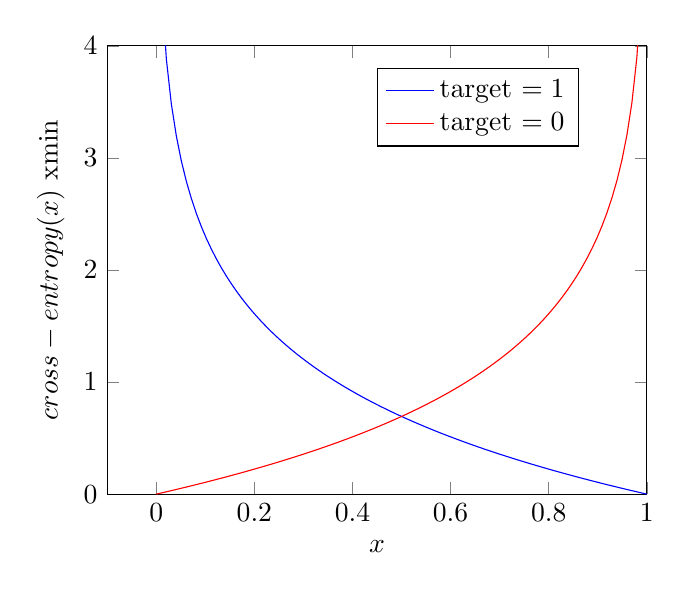
\begin{tikzpicture}
			\begin{axis}[ 
			xlabel=$x$,
			ylabel={$cross-entropy(x)$}
			xmin=0, xmax=1,
			ymin=0, ymax=4,
			legend style={at={(0.5,0.95)},anchor=north west}
			] 
			\addplot[domain=-0.01:1, color=blue, samples=100] 
				{-ln(x)};
			\addplot[domain=0:1, color=red, samples=100]
				{-ln(1 - x)};
			\addlegendentry{target $=1$}
			\addlegendentry{target $=0$}
			\end{axis}
			\end{tikzpicture}
			\caption{Binary Cross-Entropy}
			\label{fig:cross-entropy:1}
	\end{figure}
	
	\subsubsection{Mean-Squared Error (L2)}
	Mean-squared error is used for regression tasks, where the objective is to predict a quantitative value rather than a measure of probability. As L2 loss minimises the average error between the predictions $\bm{\hat{y}}$ and targets $\bm{y}$, the system learns to make predictions which lie in the mean position of these, which is generally ideal for regression tasks where there is one solution.\\
	\begin{equation} \label{mean-squared-error:1}
	 L2(\hat{\bm{y}}, \bm{y}) = \sum_{k=1}^{N}(y_k - \hat{y}_k)^2
	\end{equation}
	
	\section{Neural Networks}
	Artifical Neural Networks (\textit{ANNs}) are machine learning systems loosely inspired by the functioning of the biological neural networks of the brain. They are composed of artificial neurons which transmit signals from one another in the form of a non-linear function of the sum of the incoming inputs. ANNs model unknown functions of arbitrary complexity, with their representational power a function of their size. \par
	If we look at the structure of the simplest neuron possible $f_1$ (figure \ref{fig:neurons:1}a) we see that it is composed of two components - a weight $w_1$ and a bias $b_1$. Passing a value $x$ through a neuron $f_1$ is equivalent to computing the linear function $f_1(x) = w_1x + b_1$. The output of a neuron is known as its ``activation'' -- how activated the neuron was given that input.
	If the outputs of this neuron are then passed into a similar neuron $f_2$, we end up with the composite function 
	\begin{align}
	 (f_2\circ f_1)(x) &= (w_2(w_1x + b_1) + b_2) \\
	 &= w_2w_1x + b_1w_2 + b_2	
	\end{align}
	which is still a linear function of $x$. This is true for any number of sequential neurons, meaning that any composition of linear neurons is only as good as a single neuron. Having the capacity to produce linear relationships is only useful if the function being modelled is, itself, a linear function. For more complex modelling tasks -- which are encountered more often than not -- non-linearities need to be introduced into the network. In making a neuron a non-linear function, the problem with composite functions noted above no-longer exists; adding additional neurons increases the representational power of the model. \par
	
	\subsection{Activation Functions / Non-Linearities}
	Activation functions (also known as non-linearities) are a critical component of neural networks as they add the capacity to model non-linear relationships. The inspiration for activation functions is drawn -- once again -- from the operation of biological neural networks, whereby neurons are only ``activated'' given sufficient input signal. In modern neural networks there are only a few activation functions regularly used: \par


	\begin{itemize}
		\item\textbf{Sigmoid} $= \frac{1}{1 + e^{-x}}$ : The Sigmoid activation function (also known as the \textit{logistic function}) has the nice property that $(\forall x \in \mathbb{R}) Sigmoid(x)\in(0, 1)$ which is useful as a way of normalising values, especially when the output is to be interpreted as a probability.
		
		\item\textbf{TanH} $= \frac{e^{2x} - 1}{e^{2x} + 1}$ : The hyperbolic tangent function is similar to sigmoid, but maps numbers to the range $(-1, 1)$.
		
		\item\textbf{ReLU} $= \begin{cases}
		0, & \text{if } x < 0 \\
		x, & \text{if } x \ge 0 \\
		\end{cases}$
		The Rectified Linear Unit maps numbers to the range $[0, \infty)$ and has the advantage that it is much more computationally efficient than the above two activation functions; in most cases it yields better results.
		\item\textbf{Leaky ReLU} $= \begin{cases}
		0.01x, & \text{if } x < 0 \\
		x, & \text{if } x \ge 0 \\
		\end{cases}$
		The Leaky Rectified Linear Unit operates like ReLU, but allows numbers less than zero to ``leak'' through - this is helpful during \textit{backpropogation}, which is discussed at length in section \ref{backprop:1}.
	\end{itemize}

	\subsection{Fully-Connected Layers} \label{fully-connected:1}
	The arrangement and structure of neurons discussed thus far hasn't been very practical, in that we were only considering a chain of continuous neurons one after another with only one input and output. Neurons will typically receive multiple inputs and produce a weighted sum of those inputs (fig \ref{fig:neurons:1}b). A neuron given $N$ inputs $x_i$ with weights $w_i$ and bias $b$ would then form the linear equation $w_1x_1 + w_2x_2 + ... + w_Nx_N + b$. \textit{For our purposes we will consider the activation function to be inside each neuron, although in practice they are applied in a layered manner.} \par
	For a system consisting of multiple inputs, we want to allow diverse interactions between them. This is achieved by what's known as a \textit{Fully-Connected Layer} of neurons, where each output from the previous layer is passed as input to each of the following layer's neurons. Networks are generally grouped into layers to provide a nice abstraction away from the hundreds or thousands of neurons inside. The layer architecture of neural networks means that each layer can be considered a stand-alone block, a black box with a mapping from an an arbitrary input size to an arbitrary output size. They can therefore be stacked on top of each-other to form a \textit{fully-connected neural network} - see figure \ref{fig:neurons:1}c for an example. \par
	A valid interpretation of the weights in a neural network is to consider them a measure of the importance of the inputs for the corresponding output. For example, a network which predicts the price of a house given the number of bedrooms; square metres; and the window-thickness, will likely have a very small weight for the window-thickness as it's not very \textit{important} to the price prediction. This is a very literal example, and with more complex tasks such as image classification the weights are not as easily interpretable. \par
	\begin{figure}[h]
		\centering
		\includegraphics[width=14cm]{neurons}
		\caption{Neurons and fully-connected layers}
		\label{fig:neurons:1}
	\end{figure}

	\subsection{Stochastic Gradient Descent (SGD)} \label{sgd:1}
	An ANN begins with randomly generated weights and biases $\bm{W}$ and $\bm{B}$, which are collectively referred to as the ``parameters'' or ``weights'' and indicated by $\bm{\theta}$. The objective of an ANN is to select weights $\bm{\theta}$ that minimise the error computed by the loss function $\mathcal{L}$ (section \ref{loss:1}). Linear functions $f(\bm{x}, \bm{\theta})$ can be minimised by analytical techniques, but complex neural networks must be iteratively optimised by numerical methods. \par
	With the loss between a prediction $\hat{y}$ and target $y$, we can compute the gradients of the parameters and make a small step in the direction which will reduce the loss for the given example (see figure \ref{fig:grad-descent:1}). When performing this operation over the entire data-set at once, this is known as gradient descent. This is usually not an option as the computational resources required for full gradient descent are prohibitive. If we instead repeat this operation for different examples until we have stabilised the loss to a low value, we have Stochastic Gradient Descent. The most common variant to this technique is known as Batch Gradient Descent, where instead of computing the loss and performing an update to the parameters on a per-example basis, the process is applied once per \textit{batch} of examples. It facilitates more stable learning, as the loss doesn't fluctuate as much as between single examples. Batch Gradient Descent is the basis for most ANN optimisation, although we'll discuss modern variants in section \ref{optimizers:1}. \par
		\begin{figure}[h]
		\centering
		\includegraphics[width=9cm]{graddescent}
		\caption{Gradient descent updates}
		\label{fig:grad-descent:1}
	\end{figure}

	\subsection{Gradients and Backpropagation} \label{backprop:1}
	We shall consider a general ANN $\sigma$ with $2$ fully-connected layers $f_1, f_2$ parameterised by $\bm{\theta} = \{\bm{\theta}_1, \bm{\theta}_2\}$ which can be represented as:
	\begin{align} \label{gradients:1}
	 \bm{\hat{y}} = \sigma(\bm{x}, \bm{\theta}) = f_2(f_1(\bm{x},  \bm{\theta}_1), \bm{\theta}_2)
	\end{align}
	That is, the input $\bm{x}$ is fed through layer $f_1$ then $f_2$. We will also consider an arbitrary loss function $\mathcal{L}$ which compares the predictions $\bm{\hat{y}}$ with targets $\bm{y}$ and produces a scalar loss value:
	\begin{align}
	 \mathcal{L}(\bm{\hat{y}}, \bm{y})
	\end{align}
	As the input $\bm{x}$ and target $\bm{y}$ is fixed, we may only change the parameters $\bm{\theta}$ to improve the loss. As explained in section \ref{sgd:1}, we wish to make incremental changes to our parameters where each change decreases our loss value. We do so by computing the gradient of the parameters with respect to the loss value:
	\begin{align}
	 \frac{\partial\mathcal{L}(\bm{\hat{y}},\bm{y})}
	 {\partial\bm{\theta}}
	\end{align}
	If we are to find the gradients of the loss function with respect to the final layer's weights, we will have the equation
	\begin{align}
	\frac{\partial\mathcal{L}(\bm{\hat{y}},\bm{y})}
	{\partial\bm{\theta}_2}
	\end{align}
	which is considered to be easily calculable. However, if we wish to find the gradient of weights further towards the start of the network, we cannot work those out directly and instead need to make use of the differentiation chain rule: \par
	\begin{align}
	\frac{\partial f}{\partial x} = \frac{\partial f}{\partial u} \frac{\partial u}{\partial x}
	\end{align}
	To find the gradient of the loss function with respect to the first layer's weights, and considering that $\frac{\partial\mathcal{L}(\bm{\hat{y}},\bm{y})}
	{\partial\bm{\theta}_2}$ is calculable, we simply need apply the chain rule as such:
	\begin{align}
	\frac{\partial\mathcal{L}(\bm{\hat{y}},\bm{y})}{\partial\bm{\theta}_1} =
	\frac{\partial\mathcal{L}(\bm{\hat{y}},\bm{y})}
	{\partial\bm{\theta}_2}
	\frac{\partial\bm{\theta}_2}
	{\partial\bm{\theta}_1} 
	\end{align}
	That is, once we know the gradient of the loss with respect to the second layer's weights, we can compute the gradient of the second layer's weights with respect to the first layer's weights and multiply the two to find the gradient of the loss with respect to the first layer's weights. This generalises to neural networks with any number of layers of differing types. This is an intuitive relationship, as we are essentially calculating the compound contribution that a change in any one parameter's value will have on the final output -- the loss.  \par
	This technique used since the 1970s \parencite{backprop} is aptly named \textit{backpropagation of error gradient}, as it involves the propagation of the gradient of the error -- or loss -- from the end of the network back. \par
	Returning to the concept of SGD (section \ref{sgd:1}) which was introduced on a conceptual level, we can now delve deeper into the application of the algorithm. Assuming that we have computed the gradient of each parameter in the network for the given examples in our batch, we can visualise this as a ``loss landscape'', whereby moving the parameters down-hill results in a reduction in the loss. Adjusting a parameter by the negative of the gradient will result in a ``step'' that moves the parameter closer to a local minimum, with the objective to reach the lowest point possible. A configurable hyper-parameter is the \textit{learning-rate}, commonly represented by $\alpha$, which is the ``size'' of the step to take - that is, the coefficient of the negative of the gradient to apply (eqn. \ref{sgd:1}). \par
	\begin{align} \label{sgd:1}
		\bm{\theta} = \bm{\theta} - \alpha \Delta_{\bm{\theta}} \mathcal{L}(\bm{\theta}, \bm{\hat{y}}, \bm{y})
	\end{align}
	\textit{For brevity we will from now write the gradient of the parameters $\bm{\theta}$ with respect to the loss function $\mathcal{L}$ as $\Delta_{\bm{\theta}} \mathcal{L}(\bm{\theta})$.} \\
	The problem that is quickly encountered is how large a value to set the learning rate $\alpha$. Too small a step and it will take a long time to reach a minimum; too large and you may over-shoot it (see figure \ref{fig:learning-rate:1}). The example in figure \ref{fig:learning-rate:1} is a very low-dimensional loss landscape where the correct direction to move seems very logical, but higher dimensional spaces with a greater number of parameters result in complex landscapes with many local minima. We also want to slow down when nearing the bottom of a minimum so we can properly reach the lowest point. If we take this into consideration, and the fact that for any mini-batch the loss landscape will be different due to noise in small sample sizes, choosing a fixed learning rate becomes problematic. In practice, many people simply set up a learning rate schedule, where they decrease the learning rate at intervals, but it is hard to get right. It is with this in mind that adaptive optimizers came about. \par
	\begin{figure}[h]
		\centering
		\includegraphics[width=10cm]{learningrate}
		\caption{Learning rate values}
		\label{fig:learning-rate:1}
	\end{figure}
	
	\subsection{Adaptive Optimizers} \label{optimizers:1}
	If we consider a data-set whereby each mini-batch has some noise but that there is an optimal parameterisation for the entire set, we could visualise the loss landscape as shifting slightly for each mini-batch, but where there is a common direction towards which most samples will lead. Standard SGD will just apply a fixed step-size for all updates which leads the parameters to oscillate along the greatest descent angle, regardless of past updates. \par
	
	\subsubsection{SGD with Momentum}
	It is with the idea of a consistent optimization direction that momentum \parencite{backprop} comes into play. This is a technique of updating parameters while taking past updates into consideration to find the ``common direction'' in which to move. This is done by using an update vector which intuitively acts like the momentum of a ball rolling down a hill. For any update step, the direction vector is updated with a scaled contribution from the current gradient direction, and that vector is used to update the parameters. It essentially dampens oscillating movement, as the direction vector compounds contributions in the same direction as given in the following equation
	\begin{align}
		\bm{v}_t &= \gamma \bm{v}_{t-1} + \alpha \Delta_{\bm{\theta}} \mathcal{L}(\bm{\theta}) \\
		\bm{\theta}_t &= \bm{\theta}_{t-1} - \bm{v}_t
	\end{align}
	where $\gamma$ is the momentum term which indicates how much movement we wish to carry forward from previous time-steps.
	
	\subsubsection{Nesterov Accelerated Gradient Descent} \label{nesterov}
	If we consider momentum to compound the previous slopes such as a ball rolling down a hill, we end up with a problem where the momentum may cause the parameters to overshoot the minimum. Nesterov Accelerated Gradient Descent \parencite{nesterov} pre-emptively considers post-step parameters and makes adjustments to the step \textit{actually} taken. It does so by approximating the position after a momentum parameter update ($\bm{\theta} - \gamma\bm{v}_{t-1}$), and computes the loss gradient not with respect to the current parameters, but to the approximate future position of the parameters. This optimisation strategy essentially glances into the future and makes a pre-emptive correction.
	\begin{align}
		\bm{v}_t &= \gamma \bm{v}_{t-1} + \alpha \Delta_{\bm{\theta}} \mathcal{L}(\bm{\theta} - \gamma\bm{v}_{t-1}) \\
		\bm{\theta}_t &= \bm{\theta}_{t-1} - \bm{v}_t
	\end{align}
	
	\subsubsection{Adagrad}
	Adagrad \parencite{adagrad} is the first of the true ``adaptive'' optimizers, in that it adjusts the learning rate on a per-parameter basis, taking past gradients into consideration. The Adagrad update rule is
	\begin{align} \label{adagrad:1}
		\theta_{t, i} &= \theta_{t-1, i} - \frac{\gamma}{\sqrt{g_{t, i} + \epsilon}} \mathcal{L}(\theta_{t, i})
	\end{align}
	where $\theta_i$ is the $i$th parameter, $\gamma$ is the learning rate, $g_i$ is the square of the sum of the squares of the gradients with respect to $\theta_i$ up to step, $\epsilon$ is a small number to avoid dividing by zero, and $\mathcal{L}(\theta_i)$ is the gradient of the loss with respect to $\theta_i$. This optimizer has the benefit that while rarely performing as well as SGD with well-chosen hyperparameters, the Adagrad's default learning rate of $0.01$ consistently yields very good results.
	
	\subsubsection{Adadelta and RMSprop}
	The accumulation of squared gradients in the denominator of Adagrad means that that the learning rate continues shrinking and eventually becomes small enough to entirely stop training. Adadelta \parencite{adadelta} seeks to resolve this by instead of storing the accumulated sum of squared gradients, keeping a running average 
	\begin{align}
		E[g^2]_{t, i} = \gamma E[g^2]_{t-1, i} + (1 - \gamma)g^2_{t, i}
	\end{align}
	and updating equation \ref{adagrad:1} to be
	\begin{align}
		\theta_{t, i} &= \theta_{t-1, i} - \frac{\gamma}{\sqrt{E[g^2]_{t, i} + \epsilon}} \mathcal{L}(\theta_{t, i})
	\end{align}
	RMSprop \parencite{rmsprop} is in effect identical to Adadelta, and were both developed to address the diminishing learning rate problem of Adagrad.
	
	\subsubsection{Adam} \label{adam:1}
	Adaptive Moment Estimation (Adam) \parencite{adam} builds from the previous adaptive optimizers by not only storing exponentially decaying averages of past squared gradients $v_{t,i}$, but by also keeping an exponentially decaying average of past gradients $m_{t,i}$ -- note the lack of the word ``squared''. 
	\begin{align}
		m_{t, i} &= \beta_1 m_{t-1, i} + (1 - \beta_1)g_{t, i} \\
		v_{t, i} &= \beta_2 v_{t-1, i} + (1 - \beta_2)g^2_{t, i}
	\end{align}
	where $\beta_1$, $\beta_2$ are hyper-parameters for the proportion of past information carried forward, with the default values typically working well in practice. Replacing $E[\bm{g}^2]$ with $\bm{v}$, $\mathcal{L}(\bm{\theta})$ with $\bm{m}$, and a small change to the square-root we end up with
	\begin{align}
		\theta_{t, i} = \theta_{t-1, i} - \frac{\gamma}{\sqrt{v_{t, i}} + \epsilon} m_{t, i}
	\end{align}	
	While not the most recent (I have omitted a few other adaptive optimizers), Adam is rapidly becoming the most frequently used optimizer for its consistent convergence and ease-of-use.
	
	\section{Dealing with Small Training Data Sets}
	Gathering a large data-set can be very costly or impractical, with neural-networks regularly requiring hundreds or thousands of examples to learn anything. Due to the difficulty in obtaining data, many approaches have been devised to allow the training of neural networks with small data-sets. \par
	
	\subsection{Overfitting}
	Likely the biggest problem with training on a small data-set is overfitting, which occurs when a model is trained on a small number of sample images. As mentioned earlier, it is desirable for a system to be shown enough images to determine which aspects of an image are characteristic of the class, and which are noise in the provided sample. Overfitting is when the model learns -- and becomes dependant on -- features specific to the training data provided that don't generalise well outside of that. \par
	The effect of overfitting is that the model achieves a significantly lower accuracy when making predictions for previously-unseen images. When training on  a small training-set, overfitting can occur very easily, as models can learn features of the training images that are specific to those alone. When working with a larger training-set, the model typically sees enough variation in provided examples to gain a good approximation for the distribution of images within each class. \par 
	A model's capacity plays a large role in appropriately fitting to a data-set. If the model has too many parameters, it can learn to ``remember'' the images for each class to make predictions, and overfitting results. If the model has too few parameters, the model cannot draw a complex-enough boundary between classes, and underfitting results. Figure \ref{fig:fitting:1} shows an example of this with a simple classification task, with three levels of fitting. The best solution is in the middle, where the decision-boundary is mostly right for the seen data-points, but isn't too tight around them. The overfitting and underfitting examples draw decision boundaries such that any new data-points are less likely to fall on their respectively correct sides. \par
	\begin{figure}[!h]
		\centering
		\includegraphics[width=14cm]{fitting}
		\caption{Levels of fitting for a simple classification task}
		\label{fig:fitting:1}
	\end{figure}

	\subsection{Transfer Learning}
	Transfer learning is a commonly employed technique of taking a neural network that has already been trained on a similar task, and adapting its weights to the new domain. For image classification, this is done by downloading a pre-trained model, replacing the final fully-connected softmax output layer with a new output layer and training on the new data-set. There isn't always a necessity to re-train the model, as a large portion may be general-enough to apply to the new dataset. Due to this, the fine-tuning of models varies between adapting all parameters in the network, to the last few layers, to only the final softmax layer.  \par
	The assumption that transfer learning hinges on is that the features learnt on a large data-set are general enough to transfer to a new, similar data-set. There are a number of well-known model architectures available for download, typically being trained on the \textit{ImageNet} image database. \par
	If the model is trained on a sufficiently large data-set it is true that the learnt features are usually general enough to receive good results after introducing relatively few samples from the new domain; but is not as effective as possible, especially when the new domain is significantly different from the old. As this approach requires the training of a model on a large source data-set, the user is either stuck with an existing model and no option to change, or must first train their own custom model on the large data-set first. This is a long, costly process which can be prohibitive. \par
	Despite these limitations, transfer learning is the most effective and frequently-used technique for training on a new data-set when the amount of labelled data is small, achieving better performance than training on the new labelled data alone. \par 

	\subsection{Few-Shot Learning}
	Few-shot learning is the ability to learn a new concept or idea from only a ``few'' examples. In the context of image-classification it is the ability to learn a new class from only a few example images. It's desirable to have a system that can learn from a small data-set, because -- as mentioned earlier -- it can be a long, costly process to label data-sets. \par
	The generalised description of few-shot learning for image classification is $N$-Way $K$-Shot learning, where $N$ is the number of classes between which the model is to make predictions; $K$ is the number of example images shown prior to having the model produce a prediction. Researchers tend to work on combinations of $N \in \{5, 10, 20\}$, $K \in \{1, 5\}$, regularly presented as one-shot and five-shot learning.
	
	\subsection{Meta Learning}
	Meta-learning can be described as ``learning how to learn'', and in the field of computer vision refers to having a system that is able to adapt rapidly to new classes or domains. The goal in standard machine learning is normally to have a system that can generalise between examples within a domain, leveraging information seen in the training data to gain a generalised understanding of the data distribution. Meta-learning contrasts this in that the goal is to learn from the relationship between a data distribution and learning itself -- instead of being tightly bound to one specific domain. This is a sensible objective, as it's a trick humans use to speed-up the learning of new information. After being shown a photo of the proverbial zebra, it is quicker and easier to approximately learn it as a ``stripy horse'' rather than consider it an entirely new concept. \par
	A ``meta-learner'' is a system that's responsible for this external-observation -- with the learner playing the usual role -- however there are many designs without a distinction between the two. Meta-learning for few-shot problems is generally categorised into three different approaches:
	\begin{itemize}
		\item \textbf{Optimization-based}: A model learns parameter update rules -- essentially replacing the role of an optimizer (section \ref{optimizers:1}) -- such that some good initial weights are modified rapidly and efficiently to perform well with the current set of images. These meta-learners typically employ an RNN (section \ref{rnn:1}).
		\item \textbf{Model-based}: A specific model architecture designed to handle few-shot problems by utilising some kind of memory unit -- typically an RNN (section \ref{rnn:1}), memory-network (section \ref{memory-nets:1}) or CNN with temporal-convolutions.
		\item \textbf{Metric-based}: A model learns a representation of the given sample images and a method by which to compare query images with the recently-provided sample(s).
	\end{itemize}

	\subsubsection{Training}
	We will now consider the environment in which the aforementioned meta-learning approaches are trained and executed. \textit{Note that this section deals only with few-shot meta-learning for image-classification}. Having the system gain a meta-understanding of a task is almost exclusively approached in an episodic manner -- each episode consisting of conditioning a model on some examples of the task, having the model make a prediction, then updating the parameters to optimise this process. \par
	As always in image-classification tasks, the data-set $\mathcal{D}$ is split into two class-disjoint sets $\mathcal{D}_{train}$ and $\mathcal{D}_{test}$, the latter a held-out set from which the model isn't allowed to learn. Additionally, as few-shot learning requires the exposure of examples before making a prediction, each of the sets is split on an episode basis into a \textit{support} set $\mathcal{D}_{S}$ and a \textit{query} set $\mathcal{D}_{Q}$. For the case of training five-way one-shot classification, the support set will consist of one image from each of five randomly selected classes from $\mathcal{D}_{train}$, with the query set consisting of one or more images drawn from the same data-set and belonging to one of the classes found in the support set (figure \ref{fig:episode:1}). The model is shown $\mathcal{D}_S$, optimizes itself for these classes, then is shown $\mathcal{D}_Q$ for which to make a prediction. The meta-learner observes this, and optimizes the process by which the learner adapts to each episode. \par
	Due to the episode-based training, where the system sees a ``new'' set of classes in each, the meta-learner learns class-agnostic relationships between the support-set and the query-set. This then means that the meta-learner must persist knowledge between episodes, effectively learning an episode-invariant learning technique. This is validated by presenting an episode from $\mathcal{D}_{test}$ without the meta-learner's observation. \par
	\begin{figure}[!h]
		\centering
		\includegraphics[width=14cm]{episode}
		\caption{An N-way K-shot training episode}
		\label{fig:episode:1}
	\end{figure}
	
	\section{Continuous Learning}
	Learning from a continuous stream of new information is a crucial milestone in the development of artificial intelligence -- especially artificial general intelligence -- as the normal offline-training procedure is impractical, and vastly different from biological neural networks. The neural networks found in the brain have the capacity for continuous learning -- the ability to learn new tasks/information without sacrificing previous skills/knowledge. ANNs don't have this capacity built-in, as the training typically occurs on a per-example (episode, image, batch, etc.) basis, with the purpose of optimising for that specific episode. It is inherent then, that a network will sacrifice its existing parameter state to perform better at the task presented. This forgetting of older knowledge when learning new information is known as \textit{catastrophic forgetting} or \textit{catastrophic interference}. \par
	Catastrophic forgetting purportedly occurs when there is representational overlap inside a network between old and new information. The easiest way to gain an understanding of the new domain is to reuse that knowledge, sacrificing performance on the previous domain. This leads to an abrupt decrease in performance on the old domain, and eventually a total loss of learned knowledge. \par
	There have been many attempts at mitigating catastrophic forgetting using as number of methods (section \ref{related-cont-learning:1}) with varying degrees of success; many drawing inspiration from the brain. Strategies include replaying older examples/tasks; freezing portions of the network's parameters; using loss functions designed to minimise forgetting; and adjusting the learning speeds for weights important for older tasks. \par
	While this literature survey is not focused on neuroscience, I will briefly mention some of the known neurophysiological functions that allow the biological neural networks to adapt quickly to new information while retaining learnt information from previous tasks. \par
	\begin{itemize}
		\item\textbf{Neurosynaptic plasticity} - The brain is particularly plastic during early development, allowing for sense-driven changes to occur on a large scale. Plasticity decreases with increasing age to provide stability, but a degree of plasticity is retained for small-scale adaptation.
		\item\textbf{Hebbian plasticity}\parencite{hebbian}\label{hebbian:1} - ``Neurons wire together if they fire together''\parencite{wirefire}. An observed pattern in the brain where synaptic efficacy (neuron firing strength) increases through persistent stimulation. Simply put, frequently used neural pathways gain strength and reduce plasticity.
		\item\textbf{Complementary learning systems} - As the brain's task is to both learn and memorise, it consists of two primary components relating to memory. The hippocampus rapidly encodes new memories into sparse representations for quick short-term recall with minimal interference, whereas the neocortex slowly encodes older memories into overlapping representations for long-term storage.
	\end{itemize}
	Researchers often return to the brain for inspiration due to its incredible capacity to deal with long-term memory without exhibiting catastrophic interference. However, the brain is far from fully understood so proposed solutions in machine learning rapidly reach a limit of practicality. \par
	
	\subsection{Class-Incremental Learning} \label{cil}
	A specific set-up for the problem of continuous learning is \emph{class-incremental learning}, where a system is introduced new classes of information in a strictly incremental manner -- class $i$ is only shown to the system after it has seen class $i-1$ in its entirety. In some variations, classes may be introduced in sizes greater than one, adding five or more classes for each increment. Class-incremental learning is a good test of a system's capacity for continuous learning, as it only has the one opportunity to learn each class distribution but is to retain that information for ``life''. \par

	\section{Modern Deep Learning Architectures} \label{modern-dl:1}
	The only ANNs we've covered as of this point are \textit{fully-connected neural networks} (section \ref{fully-connected:1}) which have a very limited capacity in terms of practical use-cases, as we'll explore in this section. \par
	
	\subsection{Convolutional Neural Networks} \label{cnn:1}s
	Let us consider a fully-connected network for classification on the popular data-set MNIST (figure \ref{fig:mnist:1}), with the raw pixel values fed in one side and a class probability distribution being output. Fully-connected layers need a single column (vector) of values as inputs, so we will first ``unwrap'' the image into a long string of pixel values before feeding it in. \par
	\begin{figure}[h]
		\centering
		\includegraphics[width=6cm]{mnist}
		\caption{Ten examples from the MNIST dataset}
		\label{fig:mnist:1}
	\end{figure}
	Each input pixel would then be mapped by a distinct neuro  n weight in the first layer, which is problematic. Following the "importance weighting" interpretation introduced in section \ref{fully-connected:1}, the network must consider each input pixel individually with regards to its importance in the classification prediction. The same input image shifted by one pixel in any direction will likely produce very different results. This problem is inherent to fully-connected layers, and is best addressed by \textit{convolutional layers}. \par
	We would instead prefer to see the image in a more global context, where we can learn about the presence or absence of features throughout the image. It's easier to describe the number eight as ``one circular thing on top of another circular thing'' than by raw pixel intensities. This was the work of hand-engineered \textit{kernels} for a long time prior to the resurgence of neural networks -- see figure \ref{fig:hand-eng-kernels:1} for examples of hand-engineered edge-detection kernels and their results. As kernels are a fundamental concept for convolutional neural networks, we'll now go into some detail. \par
	\begin{figure}[!h]
		\centering
		\includegraphics[width=8cm]{handengkernels}
		\caption{Hand-engineered edge-detection kernels}
		\label{fig:hand-eng-kernels:1}
		\textit{Image adapted from https://en.wikipedia.org/wiki/Kernel\_(image\_processing)}
	\end{figure}
	A kernel -- also known as a filter -- is a (typically square) matrix that is convolved over an input image to produce another image which contains some locally-aggregated information. It can be thought of as a window that slides over the image, seeing it in small sections. At each position the values in the input are multiplied by the corresponding point in the kernel, and the output value is their sum. Figure \ref{fig:kernel:1} shows a 3x3 kernel applied to a region of pixel values of a very small input image, and the resultant value. Their applicability to neural networks is very convenient, as all we need to do is replace the hand-engineered values with learnt weights and we have the makings of a convolutional layer. As discussed in section \ref{hand-eng:1}, hand-engineered features are usually of limited capacity, with data-driven features being more powerful. \par
	\begin{figure}[!h]
		\centering
		\includegraphics[width=12cm]{kernelimg}
		\caption{The calculation of a 3x3 kernel applied at one point}
		\label{fig:kernel:1}
	\end{figure}
	The outputs of a single kernel 3x3 convolutional layer are an image-like matrix which contains locally-aggregated information from the input image. As the kernel is 3x3 pixels, the \textit{effective receptive field} size at this point is 3x3 pixels. That is, each of the features in the outputs correspond to a 3x3 region of pixels in the inputs. If the outputs of this layer are fed into another layer of the same size, the effective receptive field size at this extra layer will be 5x5 pixels. The trend of an increasing receptive field continues for more layers, which has great consequences -- the further into a network of convolutional layers, the more global the information as the deeper filters can see more of the input image features. \par
	It's important now to discuss what ``features'' are, as they're a key concept that have a fuzzy meaning. Image features extracted by data-driven convolutional kernels are unintuitive by nature, but we can build a sufficient understanding logically. Consider that through training our network, filters will be developed that respond to important features. These features will likely be things like horizontal lines; vertical lines; and soft gradients -- simple features. Subsequent layers will be dealing with not images but extracted features, so they will be responding to \textit{combinations} of features -- things like corners and more complex edges. As we proceed further into the network, the features learnt get more complex until we have filters responding to things like dog noses, text, wheels, etc. \par
	With this knowledge that the depth of a neural network corresponds to its global understanding and its ability to learn complex features, it makes sense that modern convolutional neural networks are quite deep -- sometimes into the hundreds. For the task of image classification, the missing link in the chain is how we produce the probability over the classes -- take the outputs of the final convolutional layer, ``unwrap'' it as we did for the input image, and pass it through a fully-connected layer to produce the right number of output values. \par
	
	\subsection{Recurrent Neural Networks}\label{rnn:1}
	Nothing covered so far has had the capacity to work on variable length input and output data; Recurrent Neural Networks (RNNs) address this. We have only seen two sets of values relating to a neural network -- weights, which are the network's ``intelligence''; and activations, which are the neurons' responses to the given inputs. Only the weights persist between runs, but don't have the capacity to retain information about individual samples (if they do, they've overfit!). \par
	For a neural network with a single hidden-layer, the activations at time $t$ are $h = \sigma(\bm{W}\bm{x}_t)$ for some input $\bm{x}_t$, weights $\bm{W}$, and activation function $\sigma$. RNNs work by recursively passing their hidden state through time-steps, weighted by learnt values. This can be expressed mathematically as 
	\begin{align}
		\bm{h}_{t} = \sigma(\bm{W}\bm{x}_t + \bm{U}\bm{h}_{t-1})
	\end{align}
	where $\bm{U}$ is a learnt matrix which filters and scales the hidden state values passed between time-steps. The recurrent design of this relationship means that not only will time-step $t$ contain information from time-step $t-1$, but $t-2, t-3, ...$ Figure \ref{fig:rnn:1} shows a very simple RNN. Note that we haven't discussed how to trigger an RNN to stop -- this is purposefully omitted as it's outside the scope of this writing. \par
	By their design, RNNs are able to consider all prior information when making a prediction. This makes them a perfect candidate for time-series or arbitrary length sequence data such as text, weather predictions, speech-recognition etc.
	\begin{figure}[h]
		\centering
		\includegraphics[width=12cm]{rnn}
		\caption{A simple Recurrent Neural Network}
		\label{fig:rnn:1}
		This network maps inputs $x_i$ to outputs $y_i$ for $i \in \mathbb{N}^{[1, t]}$. Red arrows indicate error-backpropagation.
	\end{figure}
	
	\subsubsection{Exploding/Vanishing Gradients}
	When training an RNN, you typically need to see the entirety (or at least a large portion) of its outputs to compute the loss -- e.g. we can't assess how well it constructed a sentence until we can see the whole sentence. The training error is back-propagated through time from the last of the output sequence to the first of the input sequence (see the red arrows in figure \ref{fig:rnn:1}). \textit{The missing red arrow for input $x_t$ relates to the fact that we've omitted the ``stop'' trigger mentioned in section \ref{rnn:1}.} \par
	As the gradients must be passed a long way, it is easy to imagine that we may end up with compounding errors, resulting in numerical instability. Gradients are particularly susceptible to this -- with the relationship between layers being multiplicative, any consecutive operations on values less than 1 approach zero, and any consecutive operations on values greater than 1 approach $\infty$. These problems are known respectively as the vanishing gradient problem, and the exploding gradient problem. Figure \ref{fig:multi-sigmoids:1} demonstrates this problem: with the sigmoid function being applied repeatedly we see that the output values ``flatline'' with the gradient rapidly approaching zero. As the gradients are used to propagate training error, no gradient means no learning.
	\begin{figure}[h]
		\centering
		\includegraphics[width=10cm]{multi-sigmoids}
		\caption{The effects of applying the sigmoid function repeatedly}
		\label{fig:multi-sigmoids:1}
	\end{figure}
	\subsubsection{Long Short-Term Memory Units}
	Long Short-Term Memory Units (LSTMs) were proposed as a solution to the aforementioned gradient problems inherent to RNNs. They have become so prolific and successful that usage of the acronym RNN generally refers to an LSTM instead. LSTMs mitigate the exploding/vanishing gradients problem by containing information outside of the normal hidden state of the network; the vanilla RNN approach doesn't really allow for dynamic usage of the hidden state. \par
	LSTMS introduce a memory structure referred to as a \textit{gated memory cell}, which is similar to Random Access Memory on a typical computer -- information can freely be written, read, and erased out of order. However, while RAM supports digital reading/writing/erasing, LSTMs allow for \emph{analog} memory access -- data is changed and read to varying degrees in a differentiable process. There are a handful of variants on the LSTM which are growing in popularity, but as the internal workings of those, and LSTMs are too complex to discuss in this writing, swe won't explore them any further. \par
	
	\subsection{Memory Networks}\label{memory-nets:1}
	Although RNNs are designed for temporal data, they have been the architecture of choice for quite some time, as standard feed-forward networks don't have memory units. Memory networks address this by augmenting regular neural networks to have an addressable external memory unit. They operate in different manner to LSTMs, but they share the same idea gates managing the read/write/erasure of elements in their respective memory unit. We will briefly touch on how a memory network functions as it has great relevance to few-shot learning, where memory of past examples is helpful, but doesn't have a strict temporal relationship. A high-level view of memory networks (figure \ref{fig:memory-nets:1}) is as follows:
	\begin{itemize}
		\item \textbf{Memory} - An indexed array of vectors representing the currently-stored information.
		\item \textbf{I}nput map - Transforms inputs to a unified internal feature representation.
		\item \textbf{G}eneralisation component - Updates old memories given new input. Referred to as ``generalsisation'' as this is responsible for compressing and generalising old memories into new representations.
		\item \textbf{O}utput map - Produces an output given the new input and the state of memory.
		\item \textbf{R}esponse component - Converts the output into the external representation,s such as text, prediction probability distribution, etc. 		
	\end{itemize}
	Memory networks have had significant success, and offer a practical alternative to RNNs when working with any variable-length data -- time-series based or not. The functionality of their memory unit has proven to perform better with long-term memory retention than even LSTMs. \par
	\begin{figure}[h]
		\centering
		\includegraphics[width=14cm]{memory-nets}
		\caption{High-level overview of a memory network}
		\label{fig:memory-nets:1}
	\end{figure}

	\section{Summary}
	In this chapter we introduced the concept of hand-engineered features, and how neural network architectures optimise this process so human-imposed knowledge doesn't limit the capacity of a system's performance. I then explained the functionality and applications of modern deep-learning architectures including CNNs; RNNs; and Memory Networks, and the problem domains within which I will be working. In the following chapter we will build on top of the backgroudn information described here, and analyse existing works in the fields of meta-learning and continuous learning. \par
	
	\chapter{Related Works} \label{related:1}
	As the problem domain spans across few-shot meta-learning and continuous learning, there is a myriad of related works of which we will introduce and summarise a selection. We will discuss the techniques used by each with a focus on their applicability to the task of few-shot continuous learning. We will then compare the results produced by each, with a closing discussion on the feasibility of their extension to the combined task. \par

	\section{Few-Shot Meta-Learning}
	The few-shot works discussed in this section represent a cross-section of most types of solutions, but especially those that relate to the thesis proposal. The techniques are broken into three sub-categories, \emph{model based}, \emph{metric based} and \emph{optimization based} -- each of which have their perks and downfalls, which are briefly mentioned at the end of each sub-section, and compared in section \ref{works:summary}. Few-shot meta-learning generally is usually considered separate to continuous-learning, so many of the approaches found in this section are less-applicable than others in the context of the proposal in chapter \ref{proposal}.

	\subsection{Model Based} \label{related-meta-modl:1}
	Model based meta-learning techniques are those that base the solution around a specific model design. These are typically implemented with some sort of memory unit -- such as an LSTM or memory network -- though this isn't a mandatory. Basing a solution on a custom model gives more freedom to design a task-specific system, but generally suffers as it can be difficult to change the architecture for different tasks. \par
	
	\subsubsection{Learning to Learn with Backpropagation of Hebbian Plasticity}
	The technique of Miconi et. al. \parencite{ltlwbohb} uses the theory of Hebbian plasticity (section \ref{hebbian:1}) to allow for connections between highly active pairs of neurons to increase in efficacy throughout their lifetime. This is achieved by defining a time-dependant quantity they call the ``Hebbian trace'', which acts as a moving-average of pair-wise synaptic activities. Using back-propagation, they train a plasticity parameter which determines how much the Hebbian trace influences the pair's connection; once trained, this plasticity parameter is fixed. The Hebbian trace is computed during all forward-passes of the network throughout its lifetime, weighting the activations of neuron-pairs proportionate to their learned plasticity. \par
	Although the technique described is primarily for continuous learning, they also apply it to a one-shot task. The task described is a toy-problem, but shows that through utilisation of the implemented Hebbian plasticity, the model is capable of quickly adapting its learning capacity to deal with the few-shot problem domain. The Hebbian trace could very easily be added into any artificial neural network architecture as an additional learned parameter. However, this technique's effectiveness at continuous learning tasks eventually becomes limited as the network's learned internal representation still remains fixed, meaning that there is no opportunity for it to consolidate knowledge as the breadth of the problem domain grows. \par
	
	\subsubsection{One-shot Learning with Memory-Augmented Neural Networks}
	One-shot learning is approached by Santoro et. al. \parencite{oslwmann} using a memory-augmented neural network (section \ref{memory-nets:1}). Memory networks are an ideal choice for few-shot learning, as they can rapidly encode, decode and selectively forget items from their external memory unit. The typical method for accessing memory locations is to use simple ``attention'', which allows the model to learn its own strategy. The authors of this paper recognise that this may result in an attention mechanism that is better purposed to sequential data, rather than the strictly un-ordered task of few-shot learning. They propose a novel memory access module called the Least Recently Used Access (LRUA) module, which is a content-based memory writer that writes memories to either the least-used or most-recently used memory locations, depending on the network's context. \par
	This new access method garnered strong results, as it allowed the network to learn the ability to replace unnecessary information as required. They show that the technique can be applied successfully to classification and regression problems, but identified that the memory unit must be cleared between tasks, lest proactive interference may occur. It must also be acknowledged that although the LRUA module achieves increased performance, it is still a complex hand-engineered solution which is not applicable to all problem domains, and is outperformed by simpler methods such as TCML (see below).  \par
	
	\subsubsection{Meta-Learning with Temporal Convolutions}
	At its core, the work of Mishra et. al. \parencite{mlwtc} devises a method which works in a purely causal manner -- the model is only influenced by previous time-steps. This is a clearly logical set-up for few-shot learning, as the task is to make decisions (specifically -- predict the class of an image) based on a small number of previously-unseen inputs. The term ``temporal convolutions'' refers to an adaptation of standard convolutions -- which convolve over coordinates -- such that the convolutions occur through time. The architecture is a deep stack of dilated temporal-convolutional layers -- where dilation basically refers to the ``overlooking'' of previous information, so as to have a larger temporal ``view'' without requiring a larger number of parameters (see the bold black diagonal lines in figure \ref{fig:temporal:1}). \par
	\begin{figure}[h]
		\centering
		\includegraphics[width=9cm]{temporal}
		\caption{Temporal Convolutional Meta-Learner (TCML) system architecture}
		\label{fig:temporal:1}
		Support image/label pairs $(i_0,y_0), (i_1,y_1), ...$ are fed in one per time-step, then the query image without its label. Image features are extracted for each input, then the TCML outputs the label for the support image it associates with the query image.
	\end{figure}
	This approach works across many problem types including few-shot and reinforcement learning, but we will only consider few-shot learning. The inputs to the network are shuffled support images with their associated labels, and a final query image with an ``empty'' place-holder label. The model thereby learns an internal relationship between the support images and the query image, effectively computing finding the most similar. As the network uses dilated temporal-convolutions, the number $N_{support}$ of support images -- and therefore the number of classes between which the network can classify -- can be quite large, with the model needing a number of layers of $log(N_{support})$, as dilated convolutions give an exponentially-increasing temporal view.  \par
	The results obtained by this technique are encouraging, achieving state-of-the-art results across the board. As with all approaches however, there are drawbacks. Other few-shot learning techniques (optimizer based - section \ref{related-meta-opt:1}, some metric based - section \ref{related-meta-metr:1}) perform a life-long update, meaning a usable classifier is produced after presenting support examples once only -- never needing to see those examples again. TCML (and most few-shot meta-learners) don't do this -- in order to perform classification, at least one example from each class must be presented alongside every query. Therefore the system's performance rapidly degrades with respect to the number of classification categories, making it an impractical choice for continuous learning. \par
	
	\subsubsection{Meta Networks}
	The so-called \emph{MetaNet} developed by Munkhdalai et. al. \parencite{mn} is somewhat an amalgamation of meta-learning techniques including memory networks and fast weight generation -- weights that are rapidly changed or generated dependent on network inputs. There is also a clear separation between the meta-learner and the base-learner, a line that is regularly indistinct with other techniques. \par
	The base-learner is parametrised by slow weights updated via a typical learning algorithm during training, and example-level fast weights generated by the meta-learner for each input (see figure \ref{fig:metanet:1}a). The base learner computes the loss for its predictions for the support set, and gives the gradients to the meta-learner. The meta-learner takes this meta information and produces a set of fast weights for the base learner when training, as well as producing its own fast weights, as a function of the information stored in memory and the meta-information. The combination of slow weights with fast weights is shown in figure \ref{fig:metanet:1}b, where its shown that the weights work in parallel, with element-wise addition used to merge the activations. \par
	\begin{figure}[h]
		\centering
		\includegraphics[width=15cm]{metanet1}
		\caption{Meta Networks system architecture}
		\label{fig:metanet:1}
	\end{figure}
	MetaNet achieves competitive results for common one-shot learning tasks, and even demonstrates positive reverse transfer as shown in figure \ref{fig:metanet:2}. This is ideal performance for a multi-task learner as it means that the meta-learner is good at persisting task-agnostic information, while incorporating newly found information. That being said, the model architecture is very complicated, with many co-dependencies between the base-learner and the meta-learner. This complexity -- and that MetaNet introduces a large number of parameters proportional to the base-learner's size -- makes it an undesirable choice for practical applications.  \newline \newline
	\begin{figure}[h]
		\centering
		\includegraphics[width=8cm]{metanet2}
		\caption{Omniglot test accuracy change obtained while training Meta Networks on MNIST}
		\label{fig:metanet:2}
	\end{figure}
	Each of the works discussed in this section have had strong results for few-shot tasks, however none have much applicability to continuous learning, and many require complex implementations. An ideal system would allow for the adding of classes throughout time, without being restrictively difficult to implement. \par
	
	\subsection{Metric Based} \label{related-meta-metr:1}
	Metric based meta-learning solutions deal with embedding query and support images into a space and computing the similarity, or distance between them. These approaches are typically very simple and accurate, but suffer from the problem that the number of embeddings and comparisons generally grows proportionate to the number of classes. This can be partially avoided by pre-embedding support images, but means that models cannot be further trained without the embeddings rapidly degrading, making them poor candidates for continuous learning. \par
	
	\subsubsection{Siamese Neural Networks for One-Shot Image Recognition}
	The work by Koch et. al. \parencite{siamese} uses \textit{siamese neural networks} to learn an image similarity-measure. Siamese networks are a class of architectures that are primarily for the purpose of computing the similarity between pairs of images. Two images are fed separately into a network which embeds them into a vector of length 4096 (see figure \ref{fig:siamese:2}). The embeddings then have the absolute value of their difference computed, and are passed through a final fully-connected layer to produce a scalar similarity value. \par
	\begin{figure}[h]
		\centering
		\includegraphics[width=9cm]{siamese}
		\caption{Overview of a siamese neural network}
		A network embeds support image $x_s$ and query image $x_q$ into $e_s$ and $e_q$, respectively. The absolute value of the difference of the embeddings is computed, then a fully connected layer outputs a single similarity value.
		\label{fig:siamese:2}
	\end{figure}
	The above-described technique is a \emph{mostly} data-driven approach for image similarity (we'll see a fully data-driven approach when discussing \textit{Relation Network} below) however this is an incomplete description of a one-shot image classification system. The novel aspect of this work is that while training, the system's task is solely image similarity, with targets of 1 when the image pair are from the same class, and 0 otherwise. When performing classification, this similarity operation is performed for with pairs consisting of the query image and each of the support set. The prediction is simply the class corresponding to the support image with which it had the highest similarity score. \par
	This approach is very simple, achieves good results, and is well studied -- with siamese networks having been in use since as early as 1994. However the amount of forward-passes increases proportionate to the number of classes, which makes it a poor candidate for continuous learning. The approach also only considers one-shot learning, which prevents the system from learning from more than one image. Although not discussed in the research paper, there are some simple modifications that could somewhat resolve these problems. The embedding function is fixed once trained, meaning that embeddings could be stored instead of images to serve as examples of classes. This minimises the increase in computation as new classes are added and makes it a better option for continuous learning. As for the limitation to one-shot learning, the system could easily be extended to allow for multiple examples per class, with the correct class being the one that receives the most "votes" across all examples. \par
	Even with the aforementioned modifications mitigating some issues in applying this to continuous learning, some problems still persist. Although adding new classes is as simple as acquiring an image, there is no guarantee that the new classes come from the same data-distribution as what the model was trained on. The embedding network could then perform poorly and therefore damage the model's ability to accurately compute the similarity for these new classes. \par
	
	\subsubsection{Matching Networks for One Shot Learning}
	The work by Vinyals et. al. \parencite{matching} focuses on a problem encountered with previous works -- simple embedding functions work on a per-image basis, not taking into account the similarity between support classes. This is addressed by creating \emph{full context embeddings}, using an LSTM to compute $emb(x_i,S)$ for $x_i \in S$ where $S$ is the support set of images. These embeddings are then stored in external memory as in a memory network. Image queries are performed by using an LSTM as an attention mechanism over the stored embeddings and taking the class that received the greatest attention. Having full context embeddings allows the network to generalise to previously-unseen data distributions for new classes. \par
	This solution is similar to model based meta-learning, but is more likely considered a metric based approach as the class prediction is made as a function of similarity to embedded support images. The one-shot results yielded by this technique are good, but in considering an extension to continuous learning we encounter obstacles. The size of memory needs to scale proportionate to the number of classes, and the LSTM embedding/attention mechanism is rather complex. \par

	\subsubsection{Prototypical Networks for Few-Shot Learning}
	The work by Snell et. al. \parencite{prototypical} proposes a simplified approach to metric based few-shot learning, while simultaneously considering the preservation of class examples without storing the actual images. Simply put, the concept is to compute a \emph{prototypical} embedding for each of the classes, and use this to perform queries. \par
	The learnt embedding function is used to embed support examples, and the mean of the support embeddings is considered the ``prototype'' for that class. Query images are embedded in the same way, and the nearest prototype is used as the class prediction. Despite being a very simple approach, this achieved better results than aforementioned works and is quite performant, owing to the fact that a single embedding vector can be used to represent an entire class and doesn't need to be fed through the network again. This seems to be a good contender when considering the continuous learning domain, but a problem encountered is that the dimensionality of the embeddings may quickly become too small, resulting in embedding collisions; retraining of the network would be required to increase the capacity of the embeddings. \par

	\subsubsection{Learning to Compare: Relation Network for Few-Shot Learning}
	Sung et. al. \parencite{relationnet} identify that a weakness in metric based few-shot learning strategies lies in the fact that the distance/similarity calculation is pre-determined -- hand-engineered. They propose a solution with an entirely data-driven similarity module, and that allows for the classification between an arbitrary number of classes. \par
	The network consists of two simple modules (see figure \ref{fig:relation-net:1})
	\begin{itemize}
		\item\textbf{Embedding module}: A sequence of convolutional layers that produces a 3-dimensional feature map per image.
		\item\textbf{Relation module}: Given a pair of feature maps -- one each for a support image and query image -- concatenates them and applies a sequence of convolutional layers. Two fully-connected layers at the end of this module transform the output to be a single value: a similarity score.
	\end{itemize}
	The model's predicted class is the class of the support image with which the query image had the greatest similarity score. This approach allows the relation module to learn a -- possibly complex -- technique for calculating the similarity between a pair of images, rather than imposing a human understanding of similarity/distance. \par
	\begin{figure}[h]
		\centering
		\includegraphics[width=14cm]{relationnet}
		\caption{Overview of Relation Network}
		The embedding module produces 3d feature maps for each support and query images, then each combination of (support, query) embedding pairs are further processed by the relation module to produce a relation score per pair. The predicted class is the maximum of these scores.
		\label{fig:relation-net:1}
	\end{figure}
	This incredibly simple solution achieves -- as of this writing -- the best results of any one-shot/few-shot techniques and is very easy to implement. However as with most metric-based approaches, Relation Network doesn't scale well as the number of classes increase, as a forward pass through the relation module needs to occur for every class and query image pair. This very quickly becomes a performance bottle-neck, and may be preventative for a many-class, high-resolution data-set. \newline \newline
	The solutions presented in this section are generally quite simple to implement, but have problems with scaling to a large number of classes, as they require computing and comparing embedded representations for each query. This makes metric based methods an unappealing choice for continuous learning tasks, where the number of classes is -- by definition -- going to increase throughout the life of the system. \par

	\subsection{Optimization Based} \label{related-meta-opt:1}
	Optimization based solutions perform few-shot meta-learning by either learning an update rule which is substituted in place of a standard optimizer; or by learning an initial set of weights which are optimal for rapid improvement from few gradient steps. A major advantage of this technique over model based and metric based approaches is that a ready-to-go classifier is obtained after presenting the new class-examples, meaning that the model's computational complexity doesn't scale so dramatically with more classes. \par
	
	\subsubsection{Optimization as a Model for Few-Shot Learning}
	The work of Ravi et. al. \parencite{oaamffsl} identifies that the gradient descent update rule of a neural network (equation \ref{update:1}) resembles the cell-state update rule for an LSTM (equation \ref{update:2}), and considers that a standard optimizer could be replaced by an LSTM. Their approach proposes a meta-learner consisting of an instance of a shared-weight LSTM per parameter in the base-learner, such that each parameter is tracked by an LSTM with its own cell-state. A conscious decision is made to share the same weights between each instance, so as to minimize the overhead in tracking a large number of parameters. \par
	\begin{align} \label{update:1}
	\theta_{t} = \theta_{t-1}-\alpha_{t}\Delta_{\theta_{t-1}}\mathcal{L}
	\end{align}
	\begin{align} \label{update:2}
	c_{t} = f_{t}\odot c_{t-1}+\i_{t}\odot \tilde{c}_t
	\end{align}
	The results garnered make this an impressive and powerful system, but not without its caveats. The training of LSTMs is notoriously tricky -- this paper mentions several specific hyper-parameters and design choices made to obtain such results. As such, difficulties would likely be encountered when applying the technique to different architectures or problem domains. \par
	A limiting design aspect of this approach is that there is no communication between parameter LSTMs. The meta-learner's gradient updates are a function of only that specific parameter's history, therefore never allowing the meta-learner to have a ``global view'' of the model's weights or gradients. An ideal solution would allow for the modelling of relationships between parameters. \par 
	
	\subsubsection{Learned Optimizers that Scale and Generalize}
	Following on from \parencite{oaamffsl}, Wichrowska et. al. \parencite{lotsag} also apply RNNs to the task of optimization in the few-shot learning domain, but allow interactions between parameters of the network by using a layered RNN structure (see figure \ref{fig:optimizer-that-scale:1}). This gives the meta-learner a better understanding of the loss-surface, and therefore the capacity to perform more informed gradient updates. Throughout the training of the meta-learner, a good initialisation for the collection of base-learners is implicitly learnt. They also implement several other improvements inspired by modern optimizers, which shall be briefly covered here as they are of interest for the proposal in chapter \ref{proposal}.
	The implemented features inspired by optimization literature are:
	\begin{itemize}
		\item\textbf{Attention and Nesterov Momentum}: Nesterov Momentum (section \ref{nesterov}) computes gradients at future positions. Similarly they use RNN attention mechanisms to explore the loss surface ahead of the current parameter position.
		\item\textbf{Momentum on multiple time-scales}: By providing the optimizer with exponential moving averages of the gradients on several time-scales, the meta-learner has access to information about how rapidly the gradient is changing and about the degree of noise in the gradient.
		\item\textbf{Dynamic input scaling}: They provide the meta-learner with multiple metrics involving the scale of weights and gradients, thereby aiding the optimizer in becoming invariant to parameter scale.
		\item\textbf{Decomposition of output into direction and step-length}: They separate the optimizer's outputs into direction and step-length, and give it no access to the learning rate so it is forced to learn from the history of gradients, instead of memorising successful learning rates.
	\end{itemize}
	\begin{figure}[h]
	\centering
	\includegraphics[width=10cm]{scalearchitecture}
	\caption{Learned Optimizers that Scale and Generalize architecture}
	The system utilizes three levels of RNNs, with shared weights between instances at each. Tensor and Global RNN instances receive the average latent state from the layer below, and pass down their outputs.
	\label{fig:optimizer-that-scale:1}
	\end{figure}
	Their experiments boast incredibly strong results, showing that -- unlike any prior methods -- this technique generalises to different problem domains, activation functions, architectures, and layer types; all previously unseen. This impressive feat is attributed to not only the layered RNN architecture, but likely the large number of aforementioned added features. Due to this complexity, this is a challenging system to re-implement and put to practice elsewhere. \par
	
	\subsubsection{Model-Agnostic Meta-Learning for Fast Adaptation of Deep Networks}
	The previous optimization-based meta-learning solutions primarily target the training of a network, but don't focus heavily on obtaining a good initial set of parameters. The approach by Finn et. al. \parencite{maml} called \emph{MAML} specifically addresses this, with the meta-learning process directly optimizing for initial parameters which can be rapidly re-trained to learn new tasks (see figure \ref{fig:maml-params:1}). There is no separate meta-learner, meaning that this technique is model-agnostic and can even be applied to different machine-learning optimization problems such as reinforcement learning. It only requires that the system is parametrized by some parameters $\bm{\theta}$, and that the loss function is smooth-enough in those parameters for gradient-based learning.
	\begin{figure}[h]
		\centering
		\includegraphics[width=6.5cm]{mamlparams}
		\caption{MAML optimization overview}
		MAML optimizes for parameters that can quickly adapt when shown new tasks. Here the new task optimal parameters are indicated by $\theta^*_i$
		\label{fig:maml-params:1}
	\end{figure}
	The meta-learning aspect of this approach is in entirely in the training algorithm (see figure \ref{fig:maml-algo:1}), with the model initialized with random weights $\theta$. MAML computes adapted parameters from each task's training set, and temporarily stores the weights $\theta'_i$ per task:
	\begin{align}
	\theta'_i = \theta - \alpha \Delta_{\theta} \mathcal{L}_{T_{i}}(f\theta)
	\end{align}
	Where $\alpha$ is a learning rate, $\mathcal{L}$ is a loss function, $f_\theta$ is a model parametrized by $\theta$, and $T_i$ is the $i$th task.
	The meta-learner objective is then to minimize the loss jointly for the updated weights and parameters using the test-set of each respective task:
	\begin{align}
	\min_\theta
	\sum_{T_i} \mathcal{L}_{T_{i}}(f_{\theta'_i}) = 
	\sum_{T_i}\mathcal{L}_{T_{i}}(f_{\theta-\alpha\Delta_\theta\mathcal{L}_{T_{i}}(f_\theta)}) \label{eqn:maml}
	\end{align}
	The parameters of the model are then updated using gradient-descent, computing gradients for the loss computed in equation \ref{eqn:maml}:
	\begin{align}
	\theta \gets \theta - \beta\Delta_\theta \sum_{T_i} \mathcal{L}_{T_{i}}(f_{\theta'_i}) \label{eqn:maml2}
	\end{align}
	Although techniques which meta-learn an update rule may intuitively be more efficacious, research \parencite{universality} has shown that there is no loss of representational power when solely optimizing the initial parameters. The same research also showed that learning the initial parameters in this way is extremely resilient to over-fitting on small data-sets. The MAML algorithm yields very impressive results, with applicability to domains as varied as robotic control, reinforcement learning and computer vision. The technique allows rapid adaptation to unseen tasks, and is truly model-agnostic. The computation of equation \ref{eqn:maml2} is costly however, as it requires the calculation of second-order derivatives; it is desired to have a simpler technique in terms of computational complexity and implementation, as few libraries directly support second-derivatives. \par
	\begin{figure}[h]
		\centering
		\includegraphics[width=9cm]{mamlalgo}
		\caption{MAML training algorithm}
		MAML computes adapted parameters from each task's training set (lines 5-6) then optimizes the model's parameters with the loss of each task's test set (line 8).
		\label{fig:maml-algo:1}
	\end{figure}
	
	\subsubsection{Reptile: a Scalable Metalearning Algorithm}
	Nichol and Schulman \parencite{reptile} sought to remove the second derivative and replace it with a simpler mechanism with their development of Reptile. Reptile optimizes for parameters which can rapidly adapt to new tasks, using a simpler and more performant approach. \par
	Reptile simply computes and temporarily stores updated weights $W_i$ for each task $T_i$ in a batch. The update applied to the parameters is a down-scaled gradient step in the direction of the sum all of them. Reptile effectively performs gradient descent in the direction of a number of tasks at once, without over-fitting to any of them.
	\begin{figure}[h]
		\centering
		\includegraphics[width=6cm]{reptilealgo}
		\caption{Reptile training algorithm}
		Reptile computes updated weights per task, then performs a gradient step in the combined direction of all of them.
		\label{fig:reptile-algo:1}
	\end{figure}
	The results yielded by Reptile are similar -- but slightly poorer -- to those of MAML, but could be considered a fair trade-off for a far-simpler implementation, and better computational efficiency. Reptile has the same applicability as for MAML, as it can be applied to essentially any model/task which can be optimized via gradient descent.
	
	
	\section{Continuous Learning} \label{related-cont-learning:1}
	Continuous learning techniques vary vastly, mainly as there is no general consensus as to what the task actually is, with the only agreement being that it is a system that can learn throughout a "lifetime", and retains information about previously learnt tasks. The works discussed in this section apply very different approaches to mostly different problems, with most being partially inapplicable to real-world situations.
	
	\subsubsection{Learning to Learn with Backpropagation of Hebbian Plasticity}
	As already reviewed in section \ref{related-meta-modl:1}, the application of Hebbian plasticity to continuous learning developed by Miconi et. al. \parencite{ltlwbohb} is sensible, but limited ongoing as the model's internal representation never changes. This results in a fixed-capacity network which is highly dependant on the initial training. An ideal system would allow for parameters to change throughout the lifetime of the model to consolidate knowledge, and to learn new feature representations.
	
	\subsubsection{Learning Without Forgetting}
	A very literal approach to continuous learning, Li et. al. \parencite{lwf} attempt to mitigate catastrophic interference by considering the base model's responses to new classes of input images as targets. They do so by augmenting the model and adding a new "output head" (see figure \ref{fig:lwf:1}) for each new collection of classes introduced to the model. When training the model on these new classes, the pre-existing output heads' predicted probability distribution is recorded, and this is included in the loss calculation. \newline
	\begin{figure}[h]
		\centering
		\includegraphics[width=8cm]{lwfarchitecture}
		\caption{Learning Without Forgetting architecture}
		A new output head (orange) is added for each batch of new classes. The model's predicted class probability distribution over the old classes is recorded and incorporated into the loss function. 
		\label{fig:lwf:1}
	\end{figure}
	They utilize a loss function developed by Hinton et. al \parencite{distillation} which was designed to distil the information in a neural network; the original purpose was to compress knowledge into a smaller neural network. The loss for Learning Without Forgetting (LwF) is separated into two parts: $\mathcal{L}_{old}$ dealing with the pre-existing output heads' collective class distributions $\bm{y}_o$, and $\mathcal{L}_{old}$ dealing with the new output head's class distribution $\bm{y}_n$. Cross-entropy (equation \ref{eqn:lwf:1}) is used for the new output head, and distillation loss (equation \ref{eqn:lwf:2}) for all pre-existing heads. \par
	\begin{align} \label{eqn:lwf:1}
	\mathcal{L}_{new}(\bm{y}_n,\hat{\bm{y}}_n) = -\bm{y}_n \cdot \text{log } \bm{\hat{y}}_n
	\end{align}
	\begin{align} \label{eqn:lwf:2}
	\mathcal{L}_{old}(\bm{y}_o,\hat{\bm{y}}_o) = -\sum_{i=1}^{l}\big( {y'}_{o}^{(i)} \cdot \text{log } \hat{y'}_o^{(i)}\big)
	\end{align}
	Where $\bm{\hat{y}}_n$ is the one-hot target over the new classes, $\bm{\hat{y}}_o$ is the recorded probability distribution, and $\hat{y'}_n^{(i)}$ and ${y'}_{o}^{(i)}$ are the targets and predictions over the old classes with weights increased for smaller probabilities. The training process is sensitive, so they perform a "warm-up stage" where only the parameters in the new head are trained, before training with the full loss function end-to-end. \par
	While a simple and elegant approach, they produced mixed results. LwF's performance on the new dataset is quite consistently better than its competitors, yet demonstrates arbitrarily better and worse resilience to catastrophic interference for the old data-set. This could be a result of the fact that as the technique is not meta-learnt, the training process never receives direct feedback on its performance on the original data-set. If a new data-set and old data-set are not very similar, there is nothing ensuring that the model retains an internal feature representation that is relevant to the old classes; this would lead to performance degradation over time. \par
	
	\subsubsection{Overcoming Catastrophic Forgetting with Hard Attention to the Task}
	Taking inspiration from neurology, Serr\'a et. al. \parencite{hat} devised an implementation of \emph{inhibitory synapses} -- a biological process which makes a neuron less likely to fire. They perform this by learning a task-based hard-attention mechanism (HaT), which masks the activations on a per-neuron basis. They perform a learnt embedding of the task description per layer, which acts as the gate for that layer. This teaches the network to learn sparse internal representations for each task, effectively reducing the required capacity within the network during training, and allowing for re-use of suitable feature representations. \par
	Serr\'a et. al. claim to address catastrophic interference well, stating that their technique yields reductions in forgetting of previous class information of 45 - 80\%. There is potential for the application to meta-learning tasks, though this is unexplored as of yet. A core limitation to this work is that the tasks must align in their output format; that is, each of the tasks were strictly image classification between 10 classes. Adding additional classes to the model is unsupported, and as such, its applicability to real-world continuous learning is quite limited. \par
	
	\subsubsection{Gradient Episodic Memory for Continual Learning}
	Long
	Gradient Episodic Memory (GEM), proposed by Lopez-Paz et. al. \parencite{gem} considers storing examples in memory to mitigate catastrophic forgetting. They store and compute loss for the $m$ most recently-seen examples from each task, with a total memory budget of $M=mT$ for $T$ distinct tasks. Storing examples for "replay" is a long-established technique, and isn't a true method of knowledge retention. GEM evicts memories on a least-recently-used basis, the model would quickly over-fit if the parameters were to be repeatedly optimized for everything in memory, seeing each example $m+1$ times before eviction. GEM side-steps this by instead minimising the loss with the constraint that loss for old examples cannot increase. \par
	\begin{figure}[h]
		\centering
		\includegraphics[width=11cm]{gem}
		\caption{GEM gradient proposal example}
		When gradients computed for new examples and memories agree (a), they are accepted; when they disagree (b), a new gradient is proposed (c) that satisfies the constraints.
		\label{fig:gem:1}
	\end{figure}
	Minimising with constraints is an unconventional technique, and is posed as a per-parameter vector-direction constraint. They first compute the gradient for each parameter for the given example, then similarly compute the gradient for each example stored in memory. If the direction of the proposed gradient step doesn't point in the same direction as the gradient computed from memory (figure \ref{fig:gem:1}), they adjust the update direction to satisfy both directions. This can be seen as not directly optimizing towards a loss minimum for the memories, but as never adjusting parameters away from this minimum. \par
	This method demonstrates a strong reduction in catastrophic interference, but has two problems which cause the practicality of this method is questionable. It involves -- in a very literal sense -- storing old examples and replaying them, which goes against the idea of a true continuous learner and grows rapidly as the number of tasks increase. Secondly, this technique doesn't allow for a varied number of classes between classification tasks which limits it to only tasks with the same output format. \par
	
	\subsubsection{Overcoming Catastrophic Forgetting}
	Kirkpatrick et. al. \parencite{ewc} propose a solution for continuous learning by designing a loss function that ties parameters to a space in which the model performed well on a previous task. They introduce an algorithm referred to as Elastic Weight Consolidation (EWC), which slows down learning on weights based on how important they are to previously seen tasks, and gives learning trajectories to maintain optimal performance (figure \ref{fig:ewc:1}). They essentially seek to find a set of good parameters for a new task that is close to good parameters for previous tasks. \par
	\begin{figure}[h]
		\centering
		\includegraphics[width=7cm]{ewc}
		\caption{Elastic Weight Consolidation parameter updates}
		EWC causes training trajectories which maintain performance on old tasks.
		\label{fig:ewc:1}
	\end{figure}
	They use a Fischer information matrix $F$, which is effectively an analytical tool for estimating the importance of the parameters $\bm{\theta}$. They then use this to weight the loss of a quadratic function which constrains the parameters to stay in the region of good performance for previous tasks $A$. As the function is quadratic, the parameters are anchored to $\theta_{A,i}^*$ as by a spring, forcing the trajectory shown in figure \ref{fig:ewc:1}. The loss function then, is:
	\begin{align}
   	\mathcal{L}(\theta) = \mathcal{L}_B(\theta) + \sum_{i} \frac{\lambda}{2} F_i (\theta_i - \theta_{A,i}^*)^2	
	\end{align}
	where $\mathcal{L}_B$ is the loss for a new task, and the sum is the loss of the parameters, which elastically constrain the parameters to a space near good performance on task $A$. \par
	Given that the solution can be implemented by simply computing a Fischer information matrix and amending the loss function, it's a highly attractive technique. That being said, although it's generalisable to most parametrized machine-learning systems, as with most other techniques it doesn't allow for a varied number of classification categories between tasks. 
	
	\section{Summary} \label{works:summary}
	In this chapter we have discussed works related to the domains of few-shot and continuous learning, and considered their feasibility to be extended to the joint-task of few-shot continuous learning. A summary of the results are shown in table \ref{fig:table:1}, where we see that there is no ideal technique. As the task at hand is a combination of both few-shot and continuous learning, we consider
	In this chapter we have discussed works related to the domains of few-shot and continuous learning. As the task at hand is a combination of both of these areas, we have also considered their feasibility to be extended to the joint task. A summary of the results shown in table \ref{fig:table:1} shows that there is no ideal technique. \par
	As expected, the methods that designed for few-shot learning are consistently applicable to few-shot tasks; we do, however see that none of the approaches could be considered entirely applicable to continuous learning. The reasons vary between techniques, ranging from entirely incompatible to functional to a limited capacity. \par
	Surprisingly, the continuous learning works are largely incompatible with our desired subset of continuous learning -- that is, the addition of an arbitrary number of classes. Most don't allow arbitrary numbers of classes to be added, with the only compatible method (Learning without Forgetting) having no capacity for few-shot learning. \par
	The problem discovered then, is that not only has continuous learning with an arbitrary number of added classes not been thoroughly studied, but that there is a large gap in pre-existing works which combine few-shot and continuous learning. This leaves us with a rather un-addressed -- yet important -- class of machine-learning problems. Having recognised the shortcomings of other approaches, in the next chapter we will propose a solution which attempts to address the outlined concerns. \par
	\begin{table}[h]
		\centering
		\includegraphics[width=17cm]{table}
		\caption{Related works comparison}
		\label{fig:table:1}
		Validation-set accuracy and feasibility of application to few-shot and continuous learning for related works. Entries are empty where no results are reported.
	\end{table}

	\chapter{Proposal} \label{proposal}
	As discovered in the previous chapter, there is a gap in the research of continuous learning problems; particularly that of designing a system which is readily applicable to real-world continuous learning problems. The discussed works cover different facets of continuous learning, but none enable the ability to repeatedly augment an image classifier to increase the number of serviceable classes. \par
	A repeatable process to extend a neural network is very appealing, as it minimises the amount of computation required to grow a network's capacity, and removes the need to retain old training examples -- both of which are often a critical limitation in the use of neural networks in production.
	
	\section{Problem Definition}
	The task is to take a model which has been trained to classify $n$ classes $\bm{X}_S = {X_S^1, X_S^2, ..., X_S^n}$, and using only the model's weights and a small number of examples from $m$ disjoint classes $\bm{X}_T = {X_T^1, X_T^2, ..., X_T^m}$, produce a model which can perform well on the combined set of classes $\bm{X}_S \cup \bm{X}_T$.
	Furthermore, an important facet of the task to not only facilitate the addition of classes to a model, but to make the function repeatable, such that a model can be continuously extended throughout its lifetime. \par
	While the relatively recent resurgence of meta-learning techniques has prompted much research in few-shot and continuous learning, no previous works attempt this task precisely. This is largely because there is much to be done in each of these individual domains, with state-of-the-art results surpassed on a very regular basis. That being said, the efficacy of meta-learning techniques is beginning to reach a limit, meaning that more novel applications are able to be considered.	\par
	The previous work that is nearest to the proposed task is \textit{Learning without Forgetting}\parencite{lwf} -- the fact that the loss function incorporates the persistence of old knowledge means that it is a strong contender. However, there is much to be gained by applying a meta-learnt system to the task, as carrying information between models allows for more generalised knowledge. An additional benefit is that an episodic learning schema provides opportunity to perform one-shot training. \par
	
	\section{Key Terminology}
	\textit{Source classes} refer to a set of classes on which a \textit{source model} has been pre-trained without meta-learning. Similarly, a \textit{target model} is produced by extending a source model's classification ability to also include a set of \textit{target classes} -- a disjoint set of classes to those that the source model was trained on. \\
	The \textit{meta-learner} is the system which facilitates the transformation of a source model into a target model. 
	
	\section{Datasets}
	Two image-classification datasets commonly used for computer-vision experiments will be used in this project:
	\begin{itemize}
		\item \textbf{CIFAR-100}\parencite{cifar100} consists of 60,000 32x32 images in 100 classes with 600 images per class. 
		\item \textbf{miniImagenet}\parencite{ilsvr} consists of 60,000 images in 100 classes of approximately 256x256 pixels with 600 images per class.
	\end{itemize}
	These datasets are to each serve a slightly different purpose -- CIFAR-100 images are sufficiently small to allow for fast training times; miniImagenet images are higher resolution, which represent a more "real-world" set of examples. Due to this, I will utilise CIFAR-100 to test prototype solutions, before applying the same techniques to the more difficult task of miniImagenet. \par 

	\section{Data-Partitioning}
	Our task involves separating the datasets in two ways -- forming disjoint sets of classes, as well as disjoint sets of examples within each of the class sets. As our datasets both contain the same number of classes and images, we will not make a distinction between the two in this section. \par
	The splitting of classes will be primarily: 80 classes for meta-training and 20 classes for meta-testing. However, this division may need to change depending on the specific experiment. To transform a model from a 20-way predictor to a 30-way predictor we would need to have at least 30 classes in the meta-test set; more than the number of classes in our pre-determined meta-test set. \par
	Due to the limited number of examples available per class, we will not hold out a set each for validation and testing, but will instead consider only training and testing splits, for which the number of images will be 500 and 100, respectively. This split matches other users of the miniImagenet dataset. \par
	
	\section{Algorithm}
	\subsection{Overview}
	
	The proposed algorithm will consist primarily of a meta-learner $M$, which takes the weights of a source model $\bm{\theta}_S$, a set of target-class images $\bm{x}_T$, and produces a set of updates $\Delta_M$. We will first discuss what occurs during one episode, then will further clarify the episode-based training procedure. As an example in this section, we will consider a model which is being transformed from a 5-way classifier to a 10-way classifier. I.e. a case where a model with the ability to classify between 5 classes is adapted to allow for classification between 10 classes. \par
	At a high-level, the proposed system architecture (figure \ref{fig:ml:1}) consists of four stages: 
	\begin{itemize}
		\item \textbf{Gradient calculation} - Gradients are calculated for the source model using target images.
		\item \textbf{Embedding} - The weights and associated gradients for each layer are separately mapped to a fixed size matrix then stacked to form a 3d matrix with a depth of 2 -- maintaining separation between weights and gradients. The mapping is performed by ``pseudo-convolutions'' -- sliding fully-connected layers across the source-model weights, mapping each dimension to a fixed-size.
		\item \textbf{Encoding and Decoding} - The weights and gradients are convolved over and down-sampled to produce a spatially-compressed representation, which is then convolved over further and up-sampled to return to the original spatial-dimensions. This output representation will only have a depth of 1, as we desire a single update value per-parameter.
		\item \textbf{Unembedding} - This decoded representation is un-embedded to match the shapes of the input weights.
	\end{itemize}
	\begin{figure}[h]
		\centering
		\includegraphics[width=17cm]{metalearnerarchitecture}
		\caption{Meta learner architecture}
		The meta learner generates weights by embedding, encoding, decoding, and un-embedding weights and gradients.
		\label{fig:ml:1}
	\end{figure}
	A target model is produced by applying the model outputs as parameter updates to the source model. \par
	Even the best and most successful adaptive optimizers (section \ref{optimizers:1}) consider only per-parameter information, without seeing the relationship between weights within even the same layer. The intuition for the encoder-decoder based approach is that as the weights and gradients are convolved over and their spatial size decreased, the meta-learner gains a more global perspective. We work with the assumption that gaining a somewhat global perspective of parameter relationships is vital in performing a single, successful weight update. Only once the midpoint of the encoder-decoder has been reached does the meta-learner have a sufficient view of the inputs to produce meaningful updates. It is this context-based information that will allow for the dramatic changes to parameters necessary for one-shot learning. \par
	The proposed approach would be considered "optimization based", as we are dealing directly with the weights and gradients themselves. This is the only practical solution, as model based and metric based options impose restrictions on the model architecture -- which is something we aim to minimise. \par
	
	\subsection{Meta-Learner}
	The meta learner -- as stated above -- produces weight updates as a function of source parameters and target images:
	\begin{align}
	\Delta_M = M(\bm{\theta}_S, \bm{x}_T)
	\end{align}
	We will now discuss how this mapping will occur within the meta-learner.

	\subsubsection{Inputs}
	We will consider only fully-convolutional source and target models. That is, models which have no fully connected layers, and the predicted class probabilities are provided by taking the maximum value from each channel in the final convolutional layer of the network. Thus, for our 5-way classifier, the final convolutional layer will consist of 5 convolutional kernels. \par
	The first step is to add new randomly initialised weights to the source model, which grows the number of kernels in the final layer from 5 to 10. With the new weights added, with the target images we will compute the gradient of the loss between the predicted values and the correct labels with respect to the source parameters $\bm{\theta}_S$. The weights and gradients are the inputs to the meta-learner systems. \par
	
	\subsubsection{Embedding}
	Each source model layer will be embedded into a fixed-size matrix, with the weights and gradients remaining separate. Each of these fixed-size embeddings will be concatenated to build a dense block of embeddings representing the entire network and its responses to the target images. \par
	
	\subsubsection{Encoding and Decoding}
	With the weights and gradients forming a 3-dimensional volume (ignoring the batch-dimension), we will be able to use something similar to a convolutional auto-encoder. In simple terms, this means that we can shrink the spatial dimensions of the volume by applying convolutional layers -- allowing the network to rapidly gain a large effective spatial field -- then apply the inverse operations to up-sample the activations to a volume with the same spatial size as the inputs. The resultant volume will be of depth 1, as we are only interested in producing a per-parameter update and don't need to maintain the separation between weights and gradients as at the inputs. \par
	This can then be un-embedded by some learnt function back to the original layer shapes, and the produced weight updates added to the source model's parameters, resulting in a target model that can classify between 10 classes.
	
	\subsection{Training Procedure}
	The training procedure is episode-based, with images seen from both the training and test set in a single episode. The procedure during meta-training and meta-testing works in the same way, but with each using a different subset of classes. The steps performed in a single episode are (figure \ref{fig:ml:2}):
	\begin{enumerate}
		\item Randomly sample a pre-trained source model $\bm{\theta}_S$, and add randomly initialised output weights.
		\item Randomly sample a set of target classes $\bm{X}_T$, not overlapping with the source-classes.
		\item Randomly sample training images $\bm{x}_{T,train}$ and test images $\bm{x}_{T,test}$ with classes $\bm{X}_T$.
		\item Generate weight updates $\bm{\Delta}_M = M(\bm{\theta}_S, \bm{x}_{T,train})$.
		\item Build target model by adding generated weight updates $\bm{\theta}_T = \bm{\theta}_S + \bm{\Delta}_M$.
		\item (meta-training only) Perform backpropagation through meta-learner with examples from combined test sets $\bm{x}_{S,test} \cup \bm{x}_{T,test}$, thus optimising the generation of weight-updates.
	\end{enumerate}
	\begin{figure}[h]
		\centering
		\includegraphics[width=10cm]{metalearneroverview}
		\caption{Meta learner training procedure}
		\label{fig:ml:2}
	\end{figure}
	As during each episode the meta-learner sees not only a different model, but a different set of source and target classes and images, the meta-learner will learn to be invariant to each of these. I.e. it won't be dependent on a specific model, class collection, or image distribution. This allows for meaningful knowledge to be obtained throughout training, and should provide great generalisation capability. \newline \newline
	There are several design choices to be made on the way, including the specific embedding and unembedding functions, and the architecture of the encoder/decoder among other things. These will be trialled empirically through the building of the system.
	
	\section{Hyper-parameter Tuning}
	The optimizer used for the experiments will likely be Adam (section \ref{adam:1}) as it has proven to yield good results with little effort in finding an appropriate learning rate. A random search in the range of $[10^{-1}, 10^{-6}]$ will be used to find an appropriate learning rate. \par
	The initialisation of the added weights for new class outputs will be investigated; the values will likely be drawn from a normal distribution, but will need to have the mean and standard deviation selected. This will be determined empirically by either experimentation, or by matching the mean and standard deviation of the pre-existing class output weights. \par
	
	\section{Evaluation}
	Evaluation metrics for this task are as-of-yet largely undefined by others, as this is a novel problem. We will, however, define a logical extension of pre-existing metrics to apply to the problem domain. \par
	The quality of a model will primarily be measured by two components: the accuracy of the target model on the target classes, and the accuracy of the target model on the source classes. The former is a measure of the meta-learner's capacity to rapidly learn from few examples; the latter a measure of how well the meta-learner retains important information embedded in the weights. Instead of considering the precision in terms of their absolute value, we will instead compute the difference between target model and source model precision. Concretely, for a collection of images, a model will produce a number of correct (C) and incorrect (I) predictions. We can therefore compute the precision for a given model $\bm{\theta}$ on images $\bm{x}$ as in equation \ref{eqn:evaluation:1}.
	\begin{align} \label{eqn:evaluation:1}
	\text{Precision}(\bm{\theta}, \bm{x}) &= \frac{C}{C+I}
	\end{align}
	To compute the relative improvement or deterioration of performance of a model, we simply need to compute the difference in precision between a source model and corresponding target model. It is not possible to measure the source model's performance on the target classes however, as it is in the problem definition that the source model has never seen the target images. In this case, we will consider the source model precision on the source images as a de-facto baseline by which to measure the target model's performance on the target classes. The improvement score equations for source and target classes are shown in equations \ref{eqn:evaluation:2} and \ref{eqn:evaluation:3}, respectively.
	\begin{align} \label{eqn:evaluation:2}
	\text{Score}_S &= \text{Precision}(\bm{\theta}_T, \bm{x}_S) - \text{Precision}(\bm{\theta}_S, \bm{x}_S) \\
	\label{eqn:evaluation:3}
	\text{Score}_T &= \text{Precision}(\bm{\theta}_T, \bm{x}_T) - \text{Precision}(\bm{\theta}_S, \bm{x}_S)
	\end{align}
	By only considering the relative improvement of a model's performance, we don't allow the difficulty of the particular classes to distort our metrics, nor the quality of the source models.
	
	
	\section{Software}
	The implementation of this proposal will be written using the Python interface for Tensorflow\parencite{tensorflow}, Google's open-source computational framework. Tensorflow has a vast collection of neural network functions pre-written, allows for automatic differentiation, and generally provides a nice environment for deep learning. In addition, Deepmind's Sonnet\parencite{sonnet} will be used, which abstracts some of the more complex and verbose aspects by way of a light wrapper around Tensorflow. Graphing and result logging will be done using Tensorboard, a visualisation tool included with Tensorflow. \par
	
	\section{Hardware}
	As deep-learning is a computationally expensive task, a computer with a high-end modern GPU is required. A computer meeting these specification has already been required, consisting of two 8GB Nvidia GTX 1080 graphics cards, a quad-core processor and 64GB of memory. The data-sets used are relatively small -- collectively of approximately 3.5GB -- so hard-drive space is not a factor that requires consideration.  \par
	
	\section{Proof of Concept}
	\TODO{I'll put something here a bit later... need to fix the current implementation!}
	
	\section{Extension Work}
	The solution proposed in this chapter is applicable only to a fixed number of source and target classes. That is, a meta-learner trained to adapt a network from 10 to 15 classes cannot be applied to the task of adapting a network from 15 to 20 classes. Although it is recognised that this limitation reduces the solution's applicability to real-world cases, the primary goal is to successfully perform this task. Generalisation will be left as an extension to this original proposal. \par
	
	\section{Summary}	
	We have now formalised the specific continuous few-shot learning task that we wish to address, and outlined a proposal for the intended solution. The implementation of the proposed solution -- even if unsuccessful -- will provide great insight into the problem-domain, and explore the limitations of meta-learning techniques for neural networks.

	\printbibliography
	
	


\end{document}
